\documentclass[11pt]{article}
\usepackage[utf8]{inputenc}
\usepackage{algorithm}
\usepackage{algorithmicx}
\usepackage[noend]{algpseudocode}
\usepackage{amsmath}
\usepackage{amssymb}
\usepackage{eucal}
\usepackage{listings}
\usepackage{mathtools}
\usepackage[svgnames]{xcolor}
\usepackage{syntax}
\usepackage{textcomp}
\usepackage{cancel}

\usepackage{hyperref}
\hypersetup{
    colorlinks=true,
    linkcolor=blue,
    filecolor=magenta,      
    urlcolor=cyan,
}
\urlstyle{same}

\usepackage{tikz}
\usetikzlibrary{automata, arrows, positioning, shapes, shapes.geometric}
\tikzset{
  every state/.style={semithick, fill=gray!10}, 
  initial text={}, 
  double distance=2pt,
  ->, >=stealth', shorten >=1pt, semithick, auto, node distance=6em
}
\tikzset{elliptic state/.style={draw,ellipse,semithick,fill=gray!10}}

\newtheorem{theorem}{Theorem}
\newtheorem{definition}{Definition}

%\newcommand*{\Language}[1]{\mathcal{L}(#1)}
\newcommand*{\Language}[1]{\ensuremath{\mathcal{L}(#1)}}
\newcommand{\MyComment}{\State $\vartriangleright$\ }
\newcommand{\mylet}{\textbf{let}\ }
\newcommand{\qaccept}{q_{\mathit{accept}}}
\newcommand{\qin}{q_{\mathit{in}}}
\newcommand{\qout}{q_{\mathit{out}}}
\newcommand{\qstart}{q_{\mathit{start}}}
\newcommand{\red}[1]{\textcolor{red}{#1}}

\newcommand{\emptylist}{\ensuremath{[\:]}}
\newcommand{\emptymap}{\ensuremath{\{ \mapsto \}}}
\newcommand{\concat}{\ensuremath{+\!\!+\:}}
\newcommand{\blank}{\ensuremath{\sqcup}}
\newcommand{\var}[1]{\ensuremath{\textit{#1}}} % variables

%--- two headed arrows, see https://tex.stackexchange.com/questions/114233/no-xrightrightarrowab ---%
\makeatletter
\providecommand*{\twoheadrightarrowfill@}{%
  \arrowfill@\relbar\relbar\twoheadrightarrow
}
\providecommand*{\twoheadleftarrowfill@}{%
  \arrowfill@\twoheadleftarrow\relbar\relbar
}
\providecommand*{\xtwoheadrightarrow}[2][]{%
  \ext@arrow 0579\twoheadrightarrowfill@{#1}{#2}%
}
\providecommand*{\xtwoheadleftarrow}[2][]{%
  \ext@arrow 5097\twoheadleftarrowfill@{#1}{#2}%
}
\makeatother

\newcommand{\set}[1]{\ensuremath{\{ #1 \} }} % sets

\title{Specifications for the GAMBA Library}
\author{Erik de Vink and Wieger Wesselink}
\date{2019--2024}

\begin{document}

\maketitle

\section{Introduction}
This document contains pseudocode specifications for the GAMBA Library, see \url{https://github.com/wiegerw/gambatools}. It contains support for DFAs, NFAs, PDAs, Turing machines (using the formalism of Sipser), context free grammars and regular expressions.

\begin{definition}
A DFA or finite automaton is a 5-tuple $(Q, \Sigma, \delta, q_0, F)$ with
\begin{enumerate}
    \item $Q$ is a finite set called the states,
    \item $\Sigma$ is a finite set called the alphabet,
    \item $\delta: Q \times \Sigma \rightarrow Q$ is the transition function
    \item $q_0 \in Q$ is the start state, and
    \item $F \subseteq Q$ is the set of accept states
\end{enumerate}
Let $D = (Q, \Sigma, \delta, q_0, F)$ be a finite automaton and let $w = w_1 w_2 \cdots w_n$ be a string where each $w_i$ is a member of the alphabet $\Sigma$. Then $D$ accepts $w$ if a
sequence of states $r_0, r_1, \ldots, r_n$ in $Q$ exists with three conditions:
\begin{enumerate}
    \item $r_0 = q_0$,
    \item $\delta(r_i, w_{i+1}) = r_{i+1}$ , for $i = 0, \ldots, n - 1$, and
    \item $r_n \in F$.
\end{enumerate}
\end{definition}

\clearpage
\begin{definition}[PDA, Sipser]
A PDA or pushdown automaton is a 6-tuple $(Q, \Sigma, \Gamma, \delta, q_0, F)$ with
\begin{enumerate}
    \item $Q$ is the set of states,
    \item $\Sigma$ is the input alphabet,
    \item $\Gamma$ is the stack alphabet,
    \item $\delta: Q \times \Sigma_\varepsilon \times \Gamma_\varepsilon \rightarrow \mathcal{P}(Q \times \Gamma_\varepsilon)$ is the transition function
    \item $q_0 \in Q$ is the start state, and
    \item $F \subseteq Q$ is the set of accept states
\end{enumerate}
Let $P = (Q, \Sigma, \Gamma, \delta, q_0, F)$ be a PDA and let $w = w_1 w_2 \cdots w_m$ be a string where each $w_i$ is a member of $\Sigma_\varepsilon$. Then $P$ accepts $w$ if 
sequences of states $r_0, r_1, \ldots, r_m \in Q$ and strings $s_0, s_1, \ldots, s_m \in \Gamma^\ast$ exist that
satisfy the following three conditions. The strings $s_i$ represent the sequence of
stack contents that $P$ has on the accepting branch of the computation.
\begin{enumerate}
    \item $r_0 = q_0$ and $s_0 = \varepsilon$
    \item For $i = 0, \ldots, m - 1$, we have $(r_{i+1}, b) \in \delta(r_i, w_{i+1}, a)$, where $s_i = at$ and $s_{i+1} = bt$ for some $a, b \in \Gamma_\varepsilon$ and $t \in \Gamma^\ast$
    \item $r_m \in F$
\end{enumerate}
\end{definition}

\bigskip

\begin{definition}[PDA, Ullman]
A UPDA or pushdown automaton \`a l\'a Ullman is a 7-tuple $(Q, \Sigma, \Gamma, \delta, q_0, Z, F)$ where
\begin{enumerate}
    \item $Q$ is the set of states,
    \item $\Sigma$ is the input alphabet,
    \item $\Gamma$ is the stack alphabet,
    \item $\delta : Q \times \Sigma_\epsilon \times \Gamma \to \mathcal{P}( Q \times \Gamma^\ast )$ is the transition function,
    \item $q_0$ is the start state,
    \item $Z$ is the start symbol or stack bottom, and
    \item $F$ is the set of accepting states or final states
\end{enumerate}
\end{definition}

\noindent
If $U = (Q, \Sigma, \Gamma, \delta, q_0, F)$ be a UPDA and let $w = w_1 \cdots w_n$ be a string with $w_i \in \Sigma_\varepsilon$ for $i = 1, \ldots, n$. 
Then $U$ accepts $w$ if states $r_0, \ldots, r_n$ in~$Q$ and strings $s_0, \ldots, s_n \in \Gamma^\ast$ exist that satisfy the following three conditions. 
\begin{enumerate}
    \item $r_0 = q_0$ and $s_0 = \varepsilon$,
    \item For $i = 0, \ldots, n {-} 1$, we have $(r_{i+1}, \varrho) \in \delta(r_i, w_{i+1}, X)$, where $s_i = X\gamma$ and $s_{i+1} = \varrho \gamma$ for some $\varrho, \gamma \in \Gamma^\ast$, $X \in \Gamma$, and
    \item $r_n \in F$.
\end{enumerate}

\clearpage
\section{Algorithms overview}
In this section a list of algorithms is given that can be used as building blocks for Gamba. We assume that $D$ is a DFA, $N$ is an NFA, $r$ is a regular expression, $P$ is a PDA, $T$ is a Turing Machine (TM), $G$ is a context free grammar, $w$ is a string in $\Sigma^*$, $text$ is a string and $k$ and $n$ are natural numbers.

\begin{table}[h!]
\begin{tabular}{ |lll| } 
\hline
\textsf{dfa-accepts-word}($D,w$) & = & $w \in \Language{D}$ \\
\textsf{dfa-words-up-to-n}($D,n$) & = & $\{ w \in \Language{D} \mid |w| \leq n \}$ \\
\textsf{dfa-minimize}($D$) & = & $D'$ a minimal DFA with $\Language{D'} = \Language{D}$ \\
\textsf{dfa-quotient}($D$) & = & $D'$ a minimal DFA with $\Language{D'} = \Language{D}$ \\
\textsf{dfa-identifiable}($D_1,D_2$) & = & reachable states of $D_1$ and $D_2$ \\
&& \qquad constitute isomorphic DFAs \\
\textsf{dfa-to-gnfa}($D$) & = & $G$ a GNFA with $\Language{G} = \Language{D}$ \\
\textsf{dfa-to-regexp}($D$) & = & $r$ with $\Language{r} = \Language{D}$ \\
\textsf{parse-dfa}($\mathit{text}$) & = & $D$ the DFA corresponding to $text$ \\
\textsf{random-dfa}($\Sigma, n$) & = & $D$ a random DFA with $n$ states and symbols in $\Sigma$ \\
\hline
\end{tabular}
\caption{DFA algorithms}
\label{table:dfa-algorithms}
\end{table}

The function \textsf{dfa-quotient} is an implementation of the quotient algorithm as given by Lewis and Papadimitriou in \cite{DBLP:books/daglib/0096996}.

\begin{table}[h!]
\begin{tabular}{ |lll| } 
\hline
\textsf{nfa-epsilon-closure}($N, q$) & = & $\{ q' \in Q \mid q \xtwoheadrightarrow{\varepsilon} q' \}$ \\
\textsf{nfa-accepts-word}($N,w$) & = & $w \in \Language{N}$ \\
\textsf{nfa-words-up-to-n}($N,n$) & = & $\{ w \in \Language{N} \mid |w| \leq n \}$ \\
\textsf{nfa-repetition}($N$) & = & $N'$ with $\Language{N'} = \Language{N}^*$ \\
\textsf{nfa-concatenation}($N_1, N_2$) & = & $N$ with $\Language{N} = \Language{N_1} \circ \Language{N_2}$ \\
\textsf{nfa-union}($N_1, N_2$) & = & $N$ with $\Language{N} = \Language{N_1} \cup \Language{N_2}$ \\
\textsf{nfa-to-dfa}($N$) & = & $D$ with $\Language{D} = \Language{N}$ \\
\textsf{nfa-to-dot}($N$) & = & $text$ a graphical representation of $N$ in dot format \\
\textsf{parse-nfa-simple}($text$) & = & $N$ the NFA corresponding to $text$ \\
\textsf{random-nfa}($\Sigma, n$) & = & $N$ a random NFA with $n$ states and symbols in $\Sigma$ \\
\hline
\end{tabular}
\caption{NFA algorithms}
\label{table:nfa-algorithms}
\end{table}

\begin{table}[h!]
\begin{tabular}{ |lll| } 
\hline
\textsf{pda-accepts-word}($P,w$) & = & $w \in \Language{P}$ \\
\textsf{pda-words-up-to-n}($P,n$) & = & $\{ w \in \Language{P} \mid |w| \leq n \}$ \\
\textsf{pda-to-cfg}($P$) & = & $G$ with $\Language{P} = \Language{G}$ \\
\textsf{pda-to-push-pop}($P$) & = & $P'$ a PDA in push/pop format with $\Language{P'} = \Language{P}$ \\
\textsf{parse-pda-simple}($text$) & = & $P$ the PDA corresponding to $text$ \\
\hline
\end{tabular}
\caption{PDA algorithms}
\label{table:pda-algorithms}
\end{table}

\begin{table}[h!]
\begin{tabular}{ |lll| } 
\hline
\textsf{tm-accepts-word}($T,w$) & = & $w \in \Language{T}$ \\
\textsf{tm-words-up-to-n}($T,n$) & = & $\{ w \in \Language{T} \mid |w| \leq n \}$ \\
\textsf{parse-tm-simple}($text$) & = & $T$ the TM corresponding to $text$ \\
\hline
\end{tabular}
\caption{TM algorithms}
\label{table:tm-algorithms}
\end{table}

\begin{table}[h!]
\begin{tabular}{ |lll| } 
\hline
\textsf{gnfa-minimize}($G$) & = & $G'$ a minimal GNFA with $\Language{G'} = \Language{G}$ \\
\hline
\end{tabular}
\caption{GNFA algorithms}
\label{table:gnfa-algorithms}
\end{table}

\begin{table}[h!]
\begin{tabular}{ |lll| } 
\hline
\textsf{cfg-accepts-word}($G,w$) & = & $w \in \Language{G}$ \\
\textsf{cfg-words-up-to-n}($G,n$) & = & $\{ w \in \Language{G} \mid |w| \leq n \}$ \\
\textsf{cfg-eliminate-epsilon-rules}($G$) & = & $G'$ with epsilon rules eliminated and $\Language{G'} = \Language{G}$ \\
\textsf{cfg-eliminate-unit-rules}($G$) & = & $G'$ with unit rules eliminated and $\Language{G'} = \Language{G}$ \\
\textsf{cfg-to-dfa}($G$) & = & $D$ with $\Language{D} = \Language{G}$ \\
\textsf{cfg-to-nfa}($G$) & = & $N$ with $\Language{N} = \Language{G}$ \\
\textsf{cfg-to-chomsky}($G$) & = & $G'$  in Chomsky normal form with $\Language{G'} = \Language{G}$ \\
\textsf{parse-cfg}($text$) & = & $G$ the CFG corresponding to $text$ \\
\textsf{parse-cfg-simple}($text$) & = & $G$ the CFG corresponding to $text$ \\
\hline
\end{tabular}
\caption{CFG algorithms}
\label{table:cfg-algorithms}
\end{table}

\begin{table}[h!]
\begin{tabular}{ |lll| } 
\hline
\textsf{regexp-accepts-word}($r,w$) & = & $w \in \Language{r}$ \\
\textsf{regexp-words-up-to-n}($r,n$) & = & $\{ w \in \Language{r} \mid |w| \leq n \}$ \\
\textsf{regexp-simplify}($r$) & = & $r'$ a simplified version of $r$ with $\Language{r'} = \Language{r}$ \\
\textsf{regexp-to-nfa}($r$) & = & $N$ with $\Language{N} = \Language{r}$ \\
\textsf{parse-regexp}($text$) & = & $r$ the regular expression corresponding to $text$ \\
\textsf{parse-regexp-simple}($text$) & = & $r$ the regular expression corresponding to $text$ \\
\textsf{random-regexp}($\Sigma, n$) & = & $r$ a random regexp of size $n$ and symbols in $\Sigma$ \\
\hline
\end{tabular}
\caption{regexp algorithms}
\label{table:regexp-algorithms}
\end{table}

\clearpage

\section{DFA algorithms}

\begin{algorithm}
\small
\caption{Test if a DFA accepts a given word }
\vspace*{1ex}
{\textbf{Input}:} 
$D = (Q, \Sigma, \delta, q_0, F)$: a DFA; $w \in \Sigma^*$ a word \\
\textbf{Output:}
$w \in \Language{D}$ \\

$\textsf{dfa-accepts-word}(D, w)$:
\begin{algorithmic}[1]
\State $q := q_0$
\For {$ a \in w$}
  \State $q := \delta(q, a)$
\EndFor
\State \Return $q \in F$
\end{algorithmic}
\end{algorithm}

\begin{algorithm}
\small
\caption{Generate accepted words in a DFA up to a given length $n$}
\vspace*{1ex}
{\textbf{Input}:}
$D = (Q, \Sigma, \delta, q_0, F)$: a DFA, $n$: a natural number \\
\textbf{Output:}
$ \{ w \in \Language{D} \mid |w| \leq n \} $ \\

$\textsf{dfa-words-up-to-n}(D, n)$
\begin{algorithmic}[1]
\State $words := \emptyset$
\If { ${q_0 \in F}$ }
  \State $words := words \cup \{ \varepsilon \}$
\EndIf
\State $W := \{ (q_0, \varepsilon) \}$
\For { ${i \in [0 \ldots n)}$ }
  \State $W' := \emptyset$
  \For { $(q, word) \in W$ }
    \For { $a \in \Sigma$ }
      \State $q' := \delta(q, a)$
      \State $word' := word \concat a$
      \State $W' := W' \cup \{ (q', word') \}$
      \If { $q' \in F$ }
        \State $words := words \cup \{ word' \}$
      \EndIf
    \EndFor
  \EndFor
  \State $W := W'$
\EndFor
\State \Return $words$
\end{algorithmic}
\end{algorithm}

\clearpage

\subsection{Converting a DFA into a language equivalent regular expression}
%% Author: Erik de Vink, February 26, 2020

To convert a DFA into a language equivalent regular expression we apply the method proposed in the book of Sipser, that makes use of the concept of a generalized NFA, also referred to as a GNFA\@. See Lemma 1.60, pages 69 to~76, in the book of Sipser.

The notion of a GNFA is a generalization of that of a DFA\@. 
In the approach of Sipser a GNFA $G = (Q, \Sigma, \delta, \qstart, \qaccept)$ has a set of states~$Q$ with two different designated states $\qstart$ and~$\qaccept$, and a transition function $\delta : Q \backslash \lbrace \qaccept \rbrace \times Q \backslash \lbrace \qstart \rbrace \to \mathit{RE}_\Sigma$. 
Thus, $\qstart$~has no incoming transitions, $\qaccept$~has no outgoing transitions, while transitions are labelled with regular expressions over the alphabet~$\Sigma$ of the GNFA\@.

As usual, the class~$\mathit{RE}_\Sigma$ of regular expressions over an alphabet~$\Sigma$ is the least set containing $\textbf{0}$, $\textbf{1}$, $\textbf{a}$ for each $a \in \Sigma$ and that is closed under sum $R_1 + R_2$, concatenation $R_1 \cdot R_2$, and the Kleene star operation, also called iteration, $R^\ast$, for $R_1, R_2, R \in \mathit{RE}_\Sigma$.
Thus,
\begin{displaymath}
R \: {:}{:}{=} \: \textbf{0} \mid \textbf{1} \mid \textbf{a} \mid R + R \mid R \cdot R \mid R^\ast
\end{displaymath}
for $a \in \Sigma$.
\bigskip

\begin{algorithm}
\small
\caption{Representing a DFA as a GNFA}
\vspace*{1.0ex}
\textbf{Input}
$D = (Q, \Sigma, \delta, q_0, F)$ a DFA \\
\textbf{Output} 
$G = (Q', \Sigma, \delta', \qstart, \qaccept)$ a GNFA that is language equivalent to $D$.

\vspace{2.0ex}

$\textsf{dfa-to-gnfa}(D)$:
\begin{algorithmic}[1]
\State $Q' := Q \cup \lbrace \qstart, \qaccept \rbrace$

\For { $q \in Q'$ } \Comment { only connect $\qstart$ with $q_0$ }
  \If { $q = q_0$ }
    \State { $\delta'(\qstart,q) := \textbf{1}$ }
  \Else
    \State { $\delta'(\qstart,q) := \textbf{0}$ }
  \EndIf    
\EndFor

\For { $(q, q') \in Q \times Q$ }
  \State $\delta'(q, q') = {+}\{ \textsf{regexp}(a) \mid \delta(q, a) = q' \}$
\EndFor

\For { $q \in Q'$ } \Comment { connect each final state of $D$ to $\qaccept$ }
  \If { $q \in F$ }
    \State $\delta'(q,\qaccept) := \textbf{1}$
  \Else
    \State $\delta'(q,\qaccept) := \textbf{0}$
  \EndIf   
\EndFor

% \For { $q \in Q$ } 
%   \MyComment { only connect $\qstart$ with $q_0$ }
%   \If { $q = q_0$ }
%     \State { $\delta'(\qstart,q) := \textbf{1}$ }
%   \Else
%     \State { $\delta'(\qstart,q) := \textbf{0}$ }
%   \EndIf    
%   \MyComment { no change in transitions among states of $D$ }
%   \For { $(q, a) \in Q \times \Sigma$ }
%     \State { $\delta'(q,\delta(q, a)) := \textsf{regexp}(a)$ }
%     \MyComment{function \textsf{regexp()} casts $a \in \Sigma$ to $\textbf{a} \in \mathit{RE}_\Sigma$}
%   \EndFor
%   \MyComment { connect each final state of $D$ to $\qaccept$ }
%   \If { $q \in F$ }
%     \State { $\delta'(q,\qaccept) := \textbf{1}$ }
%   \Else
%     \State { $\delta'(q,\qaccept) := \textbf{0}$ }
%   \EndIf   
% \EndFor

\State { \Return { $G = (Q', \Sigma, \delta', \qstart, \qaccept)$ } }

\vspace*{1.0ex}
\end{algorithmic}
\end{algorithm}

\begin{algorithm}
\small
\caption{Reducing a GNFA to a 2-state GNFA}
\vspace*{1.0ex}
\textbf{Input}
$G = (Q, \Sigma, \delta, \qstart, \qaccept)$ a GNFA \\
\textbf{Output} 
2-state GNFA $G' = (\lbrace \qstart, \qaccept \rbrace, \Sigma, \delta', \qstart, \qaccept)$ \\ \qquad where $G'$, hence the regular expression $\delta'(\qstart,\qaccept)$, language equivalent to $G$.

\vspace{2.0ex}
$\textsf{gnfa-minimize}(G)$:
\begin{algorithmic}[1]

% \For { ($q \in Q \setminus \lbrace \qstart, \qaccept \rbrace$) }
%   \MyComment { for internal, possibly equal, states $\qin$ and $\qout$ different from~$q$}
%   \For { ($\qin \in Q \setminus \lbrace q, \qstart, \qaccept \rbrace, \qout \in Q \setminus \lbrace q, \qstart, \qaccept \rbrace$) }
%     \MyComment { requires operations for regular expressions }
%     \MyComment { \qquad of sequential composition and Kleene iteration }
%     \State { $\delta(\qin,\qout) := \delta(\qin,\qout) +
%       \delta(\qin,q) \cdot \delta(q,q)^\ast \cdot \delta(q,\qout)$}
%     \State { $Q := Q \setminus \lbrace q \rbrace$ }
%   \EndFor
% \EndFor

\For {$ q_{rip} \in Q - \{ q_{start}, q_{accept} \} $}
    \State $Q := Q \setminus \{ q_{rip} \} $
    \For {$ q_i \in Q - \{ q_{accept} \} $}
        \For {$ q_j \in Q - \{ q_{start} \} $}
            \State ${ \delta(q_i, q_j) := \textsf{regexp-simplify}(
             \delta(q_i, q_{rip}) \cdot \delta(q_{rip}, q_{rip})^* \cdot \delta(q_{rip}, q_j) + \delta(q_i, q_j)) }$
        \EndFor
    \EndFor
\EndFor
\State $\delta' := \{:\}$
\State $\delta'(q_{start}, q_{accept}) := \delta(q_{start}, q_{accept})$
\State $\delta'(q_{start}, q_{start}) := \textbf{0}$
\State $\delta'(q_{accept}, q_{accept}) := \textbf{0}$
\State $\delta'(q_{accept}, q_{start}) := \textbf{0}$
\State { \Return { $G' = (Q, \Sigma, \delta', \qstart, \qaccept)$ } }
\vspace*{1.0ex}
\end{algorithmic}
\end{algorithm}

\begin{algorithm}
\small
\caption{Converts a DFA to a language equivalent regular expression}
\vspace*{1.0ex}
\textbf{Input}
$D = (Q, \Sigma, \delta, q_0, F)$: a DFA \\
\textbf{Output} 
$r$: a regular expression with $\Language{r} = \Language{D}$ \\

$\textsf{dfa-to-regexp}(D)$:
\begin{algorithmic}[1]
\State $G := \textsf{dfa-to-gnfa}(D)$
\State $\textsf{gnfa-minimize}(G)$ 
\State \Return $G.\delta(G.q_{start}, G.q_{accept})$    
\end{algorithmic}
\end{algorithm}

\clearpage

\subsection{Minimization of a DFA using the table filling method}
%% Author: Erik de Vink, 19feb2020



\begin{algorithm}
\small
\caption{Minimizing a DFA}
\vspace*{1.0ex}
\textbf{Input}
DFA $D = (Q, \Sigma, \delta, q_0, F)$: 
with $Q = \lbrace q_0 ,\, \ldots ,\, q_{n{-}1} \rbrace$

\textbf{Output} 
DFA $D'$, equivalent to $D$ and minimal in number of states

\vspace{2.0ex}

$\textsf{dfa-minimize}(D)$:
\begin{algorithmic}[1]
\MyComment { initialization of the lower triangle of table, 
  a $[0..n{-}1] \times [0..n{-}1]$ matrix }
\For { $0 \leqslant i \leqslant j < n$ } \Comment Note $i \leqslant j$ rather than $i < j$
  \State table[i,j] := 
  %$(q_i \in F \land q_j \in F) \lor (q_i \notin F \land q_j \notin F)$
  $(q_i \in F \iff q_j \in F)$
\EndFor
\State
\MyComment { comparing pairs of states on (bounded) equivalence, }
\MyComment { \qquad until no change occurs }
\State changed := true
\While { changed }
  \State changed := false
  \For { $0 \leqslant i < j < n$ }
    \If { table[i,j] }
      \For { $a \in \Sigma$ }
        \State { \mylet $q_k = \delta(q_i,a)$ }
        \State { \mylet $q_\ell = \delta(q_j,a)$ }
            \If { $\neg \text{table}[\min \lbrace k,\ell \rbrace, \max \lbrace k,\ell \rbrace$] } 
            \Comment{$k$ and $\ell$ may be equal}
          \State table[i,j] := false
          \State changed := true
          \State \textbf{break } \Comment skip remaining symbols in $\Sigma$
        \EndIf
      \EndFor
    \EndIf
  \EndFor
\EndWhile
\State $D'$ := \textsf{dfa-from-table}(D,table)
\State \Return {$D'$}
\vspace*{1.0ex}
\end{algorithmic}
\end{algorithm}

\begin{algorithm}
\small
\caption{Constructing a DFA from a minimization table}
\vspace*{1.0ex}
{\textbf{Input}} 
DFA $D = (Q, \Sigma, \delta, q_0, F)$ 
with $Q = \lbrace q_0 ,\, \ldots ,\, q_{n{-}1} \rbrace$ 
and Boolean matrix table \\
If table[i,j] = true, for any $0 < i < j < n$,
then states $q_i$ and $q_j$ can be identified

\vspace*{2.0ex}

$\textsf{dfa-from-table}(D,table)$:
\begin{algorithmic}[1]
\MyComment form sets $Q_i$ of states that can be identified according to the table
\MyComment $R$ is used to see if a state is already included
\State $R := \emptyset$
\For { $0 \leqslant i < n$ }
  \If { $q_i \notin R$ }
    \State { $Q_i := \lbrace q_i \rbrace$ }
    \State { $R$ := $R \cup \lbrace q_i \rbrace$ }
    \For { $i< j < n$ }
      \If { table[i,j] }
        \State { $Q_i := Q_i \cup \lbrace q_j \rbrace$}
        \State { $R := R \cup \lbrace q_j \rbrace$}
      \EndIf
    \EndFor
  \EndIf
\EndFor
\State
\MyComment constructing minimal DFA $D'$
\State {$Q' = \lbrace \, Q_i \mid 0 \leqslant i < n \, \rbrace$ }
\State {\mylet $Q_0$ \textbf{such that} $q_0 \in Q_0$ }
\For { $Q_i \in Q'$, $a \in \Sigma$ }
  \State { $q' := \delta(q_i,a)$ }
  \State { \mylet $j$ \textbf{such that} $q' \in Q_j$ }
  \State { $\delta'(Q_i,a)$ := $Q_j$ }
\EndFor
\State {$F' = \lbrace \, Q_i \mid q_i \in F \, \rbrace$ }
\State
\State \Return { $D' = (Q', \Sigma, \delta', Q_0, F')$ }
\end{algorithmic}
\end{algorithm}

\vspace*{2.0ex}

$\textsf{dfa-identifiable}(D_1,D_2)$:
\begin{algorithm}
\small
\caption{Decide if DFAs $D_1$ and~$D_2$ constitute isomorphic DFAs}
\vspace*{1.0ex}
{\textbf{Input}} 
DFA $D_1 = (Q_1, \Sigma, \delta_1, q^1_0, F_1)$, DFA $D_2 = (Q_2, \Sigma, \delta_2, q^2_0, F_2)$

\vspace*{1.0ex}

$\textsf{dfa-isomorphic}(D_1,D_2)$:
\begin{algorithmic}[1]
\MyComment maintain boolean matrix $\mathit{matching}$
\MyComment and a set of pairs of states $\mathit{to-inspect}$

\vspace*{1.0ex}

\For{ $q_1 \in Q_1$ and $q_2 \in Q_2$ }
\State{ $\mathit{matching}(q_1,q_2) := \mathit{false}$ }
\EndFor

\vspace*{1.0ex}

\If{ $q^1_0 \in F_1 \iff q^2_0 \in F_2$ }
\State{ $\mathit{matching}(q^1_0,q^2_0) := \mathit{true}$ }
\State{ $\mathit{to-inspect} := \{ (q^1_0,q^2_0) \}$ }
\Else
\State \Return{ $\mathit{false}$ }
\EndIf

\vspace*{1.0ex}

\MyComment{ explore DFA $D_1$ }
\While{ $\mathit{to-inspect} \neq \emptyset$ }
\State{ \textbf{choose } $(q_1,q_2) \in \mathit{to-inspect}$ }
\For{ $a \in \Sigma$ }
\State{ $q'_1 := \delta_1(q_1,a)$, $q'_2 := \delta_2(q_2,a)$ }
\If{ $\mathit{matching}(q'_1,q'_2)$ }
\If{ $q'_1 \in F_1 \iff q'_2 \in F_2$ }
\State{ $\mathit{matching}(q'_1,q'_2) := \mathit{true}$ }
\State{ $\mathit{to-inspect} := \{ (q'_1,q'_2) \}$ }
\Else
\State{ \Return{ $\mathit{false}$ } }
\EndIf
\EndIf
\EndFor
\EndWhile

\vspace*{1.0ex}

\MyComment{ check if each state of $D_1$ has a unique matching state }
\For{ $q_1 \in Q_1$ }
\State{ $\mathit{count} := 1$ }
\For{ $q_2 \in Q_2$} 
\If{ $\mathit{matching}(q_1,q_2)$ }
\State{ $\mathit{count} \, {+}{=} \, 1$ }
\EndIf
\EndFor
\If{ $\mathit{count} \neq 1$ }
\State{ \Return{ $\mathit{false}$ } }
\EndIf
\EndFor

\vspace*{1.0ex}

\MyComment{ check if each state of $D_2$ has a unique matching state }
\For{ $q_2 \in Q_2$ }
\State{ $\mathit{count} := 1$ }
\For{ $q_1 \in Q_1$} 
\If{ $\mathit{matching}(q_1,q_2)$ }
\State{ $\mathit{count} \, {+}{=} \, 1$ }
\EndIf
\EndFor
\If{ $\mathit{count} \neq 1$ }
\State{ \Return{ $\mathit{false}$ } }
\EndIf
\EndFor

\vspace*{1.0ex}

\MyComment{ DFAs are isomorphic is a proper matching exists }
\State{ \Return{ $\mathit{true}$ } }
\end{algorithmic}
\end{algorithm}

%%%%%%%%%%%%%%%%%%%%%%%%%%%%%%%%%%%%%%%%%%%%%%%%%%%%%%%%%%%%%%%%%%%%%%%%%%55

\clearpage
\subsection{Minimization of a DFA using the quotient relation}

\begin{algorithm}
\small
\caption{Minimizing a DFA using the quotient equivalence relation}
\vspace*{1.0ex}
\textbf{Input}
DFA $D = (Q, \Sigma, \delta, q_0, F)$: 
with $Q = \lbrace q_0 ,\, \ldots ,\, q_{n{-}1} \rbrace$

\textbf{Output} 
DFA $D'$, equivalent to $D$ and minimal in number of states

\vspace{2.0ex}

$\textsf{dfa-quotient}(D)$:
\begin{algorithmic}[1]
\State $\mathcal{V} := \set{F, Q \setminus F }$ \Comment{$\mathcal{V}$ is the current set of equivalence classes}
  \State $\var{eq} := \emptymap$ \Comment{Maintain a mapping from states to equivalence classes in $\mathcal{V}$}
\While { \textsf{true} }

  \For{ $V \in \mathcal{V}$ }
    \For{ $v \in V$ }
      \State $\var{eq}[v] := V$
    \EndFor  
  \EndFor

  \State $\mathcal{V}' := \emptyset$ \Comment{$\mathcal{V}'$ is the next set of equivalence classes}
  \For { $V \in \mathcal{V}$ }
    \State $\mathcal{W} := \emptyset$ \Comment{$V$ is split into equivalence classes $\mathcal{W}$}
    \For { $v \in V$ }
      \State $\textsf{matched} := \textsf{false}$
      \For { $W \in \mathcal{W}$ }
        \State $\textbf{let } w \in W$
        \If { $\forall a \in \Sigma: \var{eq}[\delta(v,a)] = \var{eq}[\delta(w,a)]$ }
          \State $W := W \cup \set{v}$
          \State $\textsf{matched} := \textsf{true}$
          \State \textbf{break}
        \EndIf
      \EndFor
      \If { $\neg \textsf{matched}$ }
        \State $\mathcal{W} := \mathcal{W} \cup \set{ \set{v} }$ \Comment{Introduce a new equivalence class for $v$}
      \EndIf
    \EndFor
    \State $\mathcal{V}' := \mathcal{V}' \cup \mathcal{W}$
  \EndFor
  \If { $\mathcal{V} \neq \mathcal{V}'$}
    \State $\mathcal{V} := \mathcal{V}'$
  \Else
    \State \textbf{break}
  \EndIf
\EndWhile
\State $\delta' := \emptymap$
\For { $V \in \mathcal{V}$ }
  \State $\textbf{let } v \in V$
  \For{ $a \in \Sigma$ }
    \State $\delta'(V,a) := \var{eq}[\delta(v,a)] $
  \EndFor
\EndFor
\State $F' := \set{ V \in \mathcal{V} \mid V \cap F \neq \emptyset }$
\State $q'_0 := \var{eq}[q_0]$
\State \Return {$D' = (\mathcal{V}, \Sigma, \delta', q'_0, F')$}
\vspace*{1.0ex}
\end{algorithmic}
\end{algorithm}

\clearpage
\subsection{Minimization of a DFA using the Hopcroft algorithm}
In \cite{DBLP:journals/corr/abs-1010-5318} the following DFA minimization algorithm is given. Note that we have slightly modified the code, to get rid of the calls to unspecified functions.

\begin{algorithm}
\small
\caption{Minimizing a DFA using the Hopcroft algorithm}
\vspace*{1.0ex}
\textbf{Input}
DFA $D = (Q, \Sigma, \delta, q_0, F)$: 
with $Q = \lbrace q_0 ,\, \ldots ,\, q_{n{-}1} \rbrace$

\textbf{Output} 
DFA $D'$, equivalent to $D$ and minimal in number of states

\vspace{2.0ex}

$\textsc{Hopcroft}(D)$:
\begin{algorithmic}[1]
\State $\mathcal{P} := \set{F, Q \setminus F } \setminus \set{\emptyset}$ \Comment{The initial partition}
\State $\mathcal{W} := \emptyset$ \Comment{The waiting set}
\For{ $a \in \Sigma$ }
  \State $\mathcal{W} := \mathcal{W} \cup \set{(\min(F, Q \setminus F), a)}$
  \Comment{Initialization of the waiting set}
\EndFor
\While{ $\mathcal{W} \neq \emptyset$ }
  \State $\textbf{let } (W,a) \in \mathcal{W}$ \Comment{Take and remove some splitter}
  \State $\mathcal{W} := \mathcal{W} \setminus \set{(W,a)}$
  \State $\mathcal{P}_\text{copy} := \mathcal{P}$
    \Comment{A copy is made, since $\mathcal{P}$ is modified in the loop}
  \For{ $P \in \mathcal{P}_\text{copy}$ }
    \State $P', P'' := (W,a) | P$ \Comment{Compute the split}
    \If{ $P' = \emptyset \lor P'' = \emptyset$ }
      \State \textbf{continue}
    \EndIf
    \State $\mathcal{P} := (\mathcal{P} \setminus \set{P}) \cup \set{P', P''}$
    \Comment{Refine the partition}
    \For{ $b \in \Sigma$ } \Comment{Update the waiting set}
      \If{ $(P,b) \in \mathcal{W}$ }
        \State $\mathcal{W} := (\mathcal{W} \setminus \set{(P,b)}) \cup \set{(P',b), (P'',b)}$
      \Else
        \State $\mathcal{W} := \mathcal{W} \cup \set{(\min(P',P''), b)}$
      \EndIf
    \EndFor
  \EndFor
\EndWhile
\State $\mathcal{Q} := \mathcal{P}$ \Comment{Construct the result}
\State $\delta' := \set{(Q', a) \mapsto Q'' \mid Q', Q'' \in \mathcal{Q} \land Q' \xrightarrow{a} Q''}$
\State $Q_0 := Q \in \mathcal{Q} \textbf{ such that } q_0 \in Q$
\State $\mathcal{F} := \set{Q \in \mathcal{Q} \mid Q \cap F \neq \emptyset}$
\State \Return $D' = (\mathcal{Q}, \Sigma, \delta', Q_0, \mathcal{F})$,
\vspace*{1.0ex}
\end{algorithmic}
\end{algorithm}
with
\begin{align*}
  \min(\{P, Q\}) &= 
  \begin{cases}
     P & \text{if } (Q = \emptyset) \lor (|P| \leq |Q| \land |P| \neq \emptyset) \\
     Q & \text{otherwise}
  \end{cases} \\
  p \xrightarrow[]{a} Q &= \exists q \in Q: p \xrightarrow[]{a} q \\
  (W,a) \mid P &= ( \{w \in W \mid w \xrightarrow{a} P\}, W \setminus \{w \in W \mid w \xrightarrow{a} P\} )
\end{align*}

\clearpage
\section{NFA algorithms}

In the algorithms below we use the convention that for NFA $N = (Q, \Sigma, \delta, q_0, F)$ the function $\delta$ may be partially defined. For all inputs $(q,a)$ where $\delta$ is undefined we
assume that $\delta(q,a) = \emptyset$.

\begin{algorithm}
\small
\caption{Epsilon closure}
\vspace*{1ex}
{\textbf{Input}:}
$N = (Q, \Sigma, \delta, q_0, F)$: an NFA; $q \in Q$: a state \\
{\textbf{Output}:}
$\{ q' \in Q \mid q \xtwoheadrightarrow{\varepsilon} q' \}$ \\

$\textsf{nfa-epsilon-closure}(N, q)$:
\begin{algorithmic}[1]
\State $result := \{ q \}$
\State $todo := \{ q \}$
\While { $todo \neq \emptyset$ }
  \State $q := todo.pop()$ \Comment{$pop$ removes and returns an arbitrary element of a set}
  \State $Q_1 := \delta(q, \varepsilon) \setminus result$
  \State $result := result \cup Q_1$
  \State $todo := todo \cup Q_1$
\EndWhile
\State \Return $result$
\end{algorithmic}
\end{algorithm}

We generalize the epsilon closure to a set of states $Q$ by
\[
\textsf{nfa-epsilon-closure}(N, Q) = \bigcup \{ \textsf{nfa-epsilon-closure}(N, q) \mid q \in Q \}.
\]

\begin{algorithm}
\small
\caption{Test if an NFA accepts a given word }
\vspace*{1ex}
{\textbf{Input}:} 
$N = (Q, \Sigma, \delta, q_0, F)$: an NFA; $w \in \Sigma^*$ a word \\
\textbf{Output:}
$w \in \Language{N}$ \\

$\textsf{nfa-accepts-word}(N, w)$:
\begin{algorithmic}[1]
\State $q := \textsf{nfa-epsilon-closure}(N, q_0)$
\For {$ a \in w$}
  \State $q := \bigcup \{ \textsf{nfa-epsilon-closure}(N, \delta(q_i, a)) \mid q_i \in q \}$
\EndFor
\State \Return $q \cap F \neq \emptyset$
\end{algorithmic}
\end{algorithm}

\begin{algorithm}
\small
\caption{Generate accepted words in an NFA up to a given length $n$}
\vspace*{1ex}
{\textbf{Input}:} $N = (Q, \Sigma, \delta, q_0, F)$: an NFA, $n$: a natural number \\
\textbf{Output:}
$ \{ w \in \Language{N} \mid |w| \leq n \} $ \\

$\textsf{nfa-words-up-to-n}(N, n)$
\begin{algorithmic}[1]

\State $F_1 := \{ q \in Q \mid \textsf{nfa-epsilon-closure}(N, q) \cap F \neq \emptyset \}$
  \Comment states that can terminate
\State $result := \emptyset$
\If { $q_0 \in F_1$ }
  \State $result := result \cup \{ \varepsilon \}$
\EndIf
\State $W := \{ (q, \varepsilon) \mid q \in \textsf{nfa-epsilon-closure}(N, q_0) \}$
\For { ${0 \leq i < n}$ }
  \State $W' := \emptymap$
  \For { $(q, words) \in W$ }
    \For { $a \in \Sigma$ }
      \For { $q_1 \in \textsf{nfa-epsilon-closure}(N, \delta(q, a))$ }
        \State $words' := \{ wa \mid w \in words \}$
        \State $W'(q_1) := W'(q_1) \cup words'$
        \If { $q_1 \in F_1$ }
          \State $result := result \cup words'$
        \EndIf
      \EndFor
    \EndFor
  \EndFor
  \State $W := W'$
\EndFor
\State \Return $result$
\end{algorithmic}
\end{algorithm}

\begin{algorithm}
\small
\caption{Convert an NFA into a language equivalent DFA }
\vspace*{1ex}
{\textbf{Input}:} 
$N = (Q_N, \Sigma, \delta_N, q_N, F_N)$: An NFA \\
{\textbf{Output}:} 
$D$: a DFA with $\Language{D} = \Language{N}$\\

$\textsf{nfa-to-dfa}(N)$:
\begin{algorithmic}[1]
\State $F := \emptyset$
\State $Q_0 := \textsf{nfa-epsilon-closure}(N,q_N)$
\State $Q := \{ Q_0 \}$
\State $\delta := \{:\}$ \Comment $\{:\}$ is the empty mapping
\If { $Q_0 \cap F_N \neq \emptyset$ } 
  \State $F := F \cup \{ Q_0 \}$
\EndIf
\State $todo := [ Q_0 ]$
\While { $todo \neq \emptyset$ }
  \State $Q_1 := todo[0]$
  \State $todo := todo[1..]$
  \For { $a \in \Sigma$ }
    \State $Q_2 := \emptyset$
    \For { $q_1 \in Q_1$ }
      \State $Q_2 := Q_2 \cup \textsf{nfa-epsilon-closure}(N, \delta_N(q_1, a))$
    \EndFor
    \State $\delta(Q_1, a) := Q_2$
    \If { $Q_2 \cap F_N \neq \emptyset$ }
      \State $F := F \cup \{ Q_2 \}$
    \EndIf
    \If { $Q_2 \notin Q$ }
      \State $Q := Q \cup \{ Q_2 \}$
      \State $todo := todo \concat [Q_2]$
    \EndIf
  \EndFor
\EndWhile
\State \Return $(Q, \Sigma, \delta, Q_0, F)$
\end{algorithmic}
\end{algorithm}

\begin{algorithm}
\small
\caption{Computes the repetition of an NFA}
\vspace*{1ex}
{\textbf{Input}:} 
$N = (Q, \Sigma, \delta, q_0, F)$: an NFA \\
\textbf{Output:}
$N'$: an NFA with $\Language{N'} = \Language{N^*}$ \\

$\textsf{nfa-repetition}(N)$:
\begin{algorithmic}[1]
\State $q'_0 := \textsf{fresh-state}()$
\State $Q' := Q \cup \{ q_0 \}$
\State $F' := F \cup \{ q_0 \}$
\State $\delta' := \delta$
\For {$q \in F$}
    \State $\delta'(q, \varepsilon) := \delta'(q, \varepsilon) \cup \{ q_0 \}$
\EndFor
\State $\delta'(q'_0, \varepsilon) := \{ q_0 \}$
\State \Return $N' = (Q', \Sigma, \delta', q'_0, F')$
\end{algorithmic}
\end{algorithm}

\begin{algorithm}
\small
\caption{Computes the union of two NFAs}
\vspace*{1ex}
{\textbf{Input}:} 
$N_1 = (Q_1, \Sigma, \delta_1, q_1, F_1)$: an NFA; $N_2 = (Q_2, \Sigma, \delta_2, q_2, F_2)$: an NFA \\
\textbf{Output:}
$N'$: an NFA with $\Language{N'} = \Language{N_1} \cup \Language{N_2}$ \\

$\textsf{nfa-union}(N)$:
\begin{algorithmic}[1]
\State $q'_0 := \textsf{fresh-state}()$
\State $Q' := Q_1 \cup Q_2 \cup \{ q_0 \}$
\State $F' := F_1 \cup F_2$
\State $\delta' := \delta_1 \cup \delta_2$
\State $\delta'(q'_0, \varepsilon) := \{ q_1, q_2 \}$
\State \Return $N' = (Q', \Sigma, \delta', q'_0, F')$
\end{algorithmic}
\end{algorithm}

\begin{algorithm}
\small
\caption{Computes the concatenation of two NFAs}
\vspace*{1ex}
{\textbf{Input}:} 
$N_1 = (Q_1, \Sigma, \delta_1, q_1, F_1)$: an NFA; $N_2 = (Q_2, \Sigma, \delta_2, q_2, F_2)$: an NFA \\
\textbf{Output:}
$N'$: an NFA with $\Language{N'} = \Language{N_1} \circ \Language{N_2}$ \\

$\textsf{nfa-concatenation}(N)$:
\begin{algorithmic}[1]
\State $q'_0 := q_1$
\State $Q' := Q_1 \cup Q_2 \cup \{ q_0 \}$
\State $F' := F_2$
\State $\delta' := \delta_1 \cup \delta_2$
\For {$q \in F_1$}
    \State $\delta'(q, \varepsilon) := \delta'(q, \varepsilon) \cup \{ q_2 \}$
\EndFor
\State \Return $N' = (Q', \Sigma, \delta', q'_0, F')$
\end{algorithmic}
\end{algorithm}

\clearpage

\section{PDA algorithms}

We define a PDA state as a tuple $(q, s)$ with $q \in Q$ a state and $s \in \Gamma^*$ a stack content. We define the functions $\textsf{can-pop-push}$ and $\textsf{pop-push}$ as follows:

\[
\begin{array}{lll}
\textsf{can-pop-push}(stack, u, v) &=& (u = \varepsilon) \lor 
                (u \neq \varepsilon \land stack = stack' \concat [u] )\\
\textsf{pop-push}(stack, u, v) &=& 
  \left \{
    \begin{array}{ll}
      stack & \text{if } u = \varepsilon \text{ and } v = \varepsilon \\
      stack \concat [v] & \text{if } u = \varepsilon \text{ and } v \neq \varepsilon \\
      stack[{:}|stack|{-}1] & \text{if } u \neq \varepsilon \text{ and } v = \varepsilon \\
      stack[{:}|stack|{-}1] \concat [v] & \text{if } u \neq \varepsilon \text{ and } v \neq \varepsilon \\
    \end{array}
  \right .
\end{array}
\]

\begin{algorithm}
\small
\caption{PDA epsilon closure}
\vspace*{1ex}
{\textbf{Input}:}
$P = (Q, \Sigma, \Gamma, \delta, q_0, F)$: a PDA; $r \in Q \times \Gamma^*$: a PDA state \\
{\textbf{Output}:}
$\{ r' \in Q \times \Gamma^* \mid r \xtwoheadrightarrow{\varepsilon} r' \}$ \\

$\textsf{pda-epsilon-closure}(P, r)$:
\begin{algorithmic}[1]
\State $result := \{ r \}$
\State $todo := \{ r \}$
\While { $todo \neq \emptyset$ }
  \State $r := todo.pop()$ \Comment{$pop$ removes and returns an arbitrary element of a set}
  \State $\textbf{let } r = (p, stack)$
  \For { $u \in \Gamma_\varepsilon $}
    \State $Q_1 := \delta(p, \varepsilon, u)$
    \For { $(q, v) \in Q_1$ }
      \If { $\textsf{can-pop-push}(stack, u, v)$ }
        \State $stack' = \textsf{pop-push}(stack, u, v)$
        \State $r' := (q, stack')$
        \If { $r' \notin result$ }
          \State $todo := todo \cup \{ r' \}$
          \State $result := result \cup \{ r' \}$
        \EndIf
      \EndIf
    \EndFor
  \EndFor
\EndWhile
\State \Return $result$
\end{algorithmic}
\end{algorithm}

\begin{algorithm}
\small
\caption{Do a transition in a PDA}
\vspace*{1ex}
{\textbf{Input}:}
$P = (Q, \Sigma, \Gamma, \delta, q_0, F)$: a PDA; $a \in \Sigma$: a symbol; $r \in Q \times \Gamma^*$: a PDA state \\
{\textbf{Output}:}
$\{ r' \in Q \times \Gamma^* \mid r \xtwoheadrightarrow{a} r' \}$ \\

$\textsf{pda-do-transition}(P, a, r)$:
\begin{algorithmic}[1]
\State $\textbf{let } r = (p, stack)$
\State $result := \emptyset$
\For { $u \in \Gamma_\varepsilon $}
  \State $Q_1 := \delta(p, a, u)$
  \For { $(q, v) \in Q_1$ }
    \If { $\textsf{can-pop-push}(stack, u, v)$ }
      \State $stack' = \textsf{pop-push}(stack, u, v)$
      \State $r' := (q, stack')$
      \State $result := result \cup \{ r' \}$
    \EndIf
  \EndFor
\EndFor
\State \Return $result$
\end{algorithmic}
\end{algorithm}

We generalize the functions \textsf{pda-epsilon-closure} and \textsf{pda-do-transition}  to a set of PDA states $R$ by
\[
\begin{array}{lll}
\textsf{pda-epsilon-closure}(P, R) & = & \bigcup \{ \textsf{pda-epsilon-closure}(P, r) \mid r \in R \} \\
\textsf{pda-do-transition}(P, a, R) & = & \bigcup \{ \textsf{pda-do-transition}(P, a, r) \mid r \in R \}.
\end{array}
\]

\begin{algorithm}
\small
\caption{Test if a PDA accepts a given word }
\vspace*{1ex}
{\textbf{Input}:} 
$P = (Q, \Sigma, \Gamma, \delta, q_0, F)$: a PDA; $w \in \Sigma^*$ a word \\
\textbf{Output:}
$w \in \Language{P}$ \\

$\textsf{pda-accepts-word}(P, w)$:
\begin{algorithmic}[1]
\State $R := \{ (q_0, []) \}$
\State $R := \textsf{pda-epsilon-closure}(P, R)$
\For {$ a \in w$}
  \State $R := \textsf{pda-do-transition}(P, a, R)$
  \State $R := \textsf{pda-epsilon-closure}(P, R)$
\EndFor
\State \Return $\exists (q, stack) \in R: q \in F$
\end{algorithmic}
\end{algorithm}

\begin{algorithm}
\small
\caption{Generate accepted words in a PDA up to a given length $n$}
\vspace*{1ex}
{\textbf{Input}:} $P = (Q, \Sigma, \Gamma, \delta, q_0, F)$: a PDA, $n$: a natural number \\
\textbf{Output:}
$ \{ w \in \Language{P} \mid |w| \leq n \} $ \\

$\textsf{pda-words-up-to-n}(P, n)$
\begin{algorithmic}[1]

\State $result := \emptyset$
\State $W := \emptymap$
\State $R := \{ (q_0, \emptylist) \}$
\State $R := \textsf{pda-epsilon-closure}(P, R)$
\For { $r \in R$ }
  \State $W(r) := \{ \varepsilon \}$
  \State $\textbf{let } r = (q, stack)$
  \If { $q \in F$ }
    \State $result := result \cup \{ \varepsilon \}$
  \EndIf
\EndFor

\For { ${0 \leq i < n}$ }
  \State $W' := \emptymap$
  \For { $(r, words) \in W$ }
    \For { $a \in \Sigma$ }
      \State $R := \textsf{pda-do-transition}(P, a, r)$
      \State $R := \textsf{pda-epsilon-closure}(P, R)$
      \State $words' := \{ wa \mid w \in words \}$
      \For { $r' \in R$ }
        \State $W'(r') := W'(r') \cup words'$
        \State $\textbf{let } r' = (q', stack')$
        \If { $q' \in F$ }
          \State $result := result \cup words'$
        \EndIf
      \EndFor
    \EndFor
  \EndFor
  \State $W := W'$
\EndFor
\State \Return $result$
\end{algorithmic}
\end{algorithm}

\begin{algorithm}
\small
\caption{Converts a PDA into a language equivalent CFG}
\vspace*{1ex}
{\textbf{Input}:} 
$P = (Q, \Sigma, \Gamma, \delta, q_0, F)$: a PDA in push/pop format \\
\textbf{Output:}
$G$: a CFG with $\Language{G} = \Language{P}$ \\

$\textsf{pda-to-cfg}(P)$:
\begin{algorithmic}[1]
\State $V := \{ A_{pq} \mid (p, q) \in Q \times Q \}$
\State $R := \emptyset$
\State $\textbf{let } F = \{ q_{accept} \}$
\State $S := A_{q_0q_{accept}}$
\State $T_{push} := \emptymap$ \Comment{maps stack symbols to corresponding push transitions}
\State $T_{pop} := \emptymap$ \Comment{maps stack symbols to corresponding pop transitions}
\For {$((p, a, u), Q_1) \in \delta$}
  \For { $(q, v) \in Q_1$ }
    \If { $u = \varepsilon$ }
      \State $T_{push}[v] := T_{push}[v] \cup \{ (p, a, \varepsilon) \rightarrow (q, v) \}$
    \ElsIf { $v = \varepsilon$ }
      \State $T_{pop}[u] := T_{pop}[u] \cup \{ (p, a, u) \rightarrow (q, \varepsilon) \}$
    \EndIf
  \EndFor    
\EndFor

\For { $u \in \Gamma$ }
  \For {$ ((p, a, \varepsilon) \rightarrow (r, u), (s, b, u) \rightarrow (q, \varepsilon))
          \in T_{push}[u] \times T_{pop}[u]
       $}
     \State $R := R \cup \{ A_{pq} \rightarrow aA_{rs}b \}$
  \EndFor
\EndFor

\For { $(p, q, r) \in Q \times Q \times Q$ }
     \State $R := R \cup \{ A_{pq} \rightarrow A_{pr}A_{rq} \}$
\EndFor

\For { $p \in Q$ }
     \State $R := R \cup \{ A_{pp} \rightarrow \varepsilon \}$
\EndFor

\State \Return $G = (V, \Sigma, R, S)$
\end{algorithmic}
\end{algorithm}


\begin{algorithm}
\small
\caption{Converts a PDA into a PDA accepting on empty stack}
\vspace*{1ex}
{\textbf{Input}:}
$P = (Q, \Sigma, \Gamma, \delta, q_0, F)$: a PDA; \\
{\textbf{Output}:}
$P = (Q', \Sigma, \Gamma', \delta', q_s, F')$: a PDA accepting on empty stack
\begin{algorithmic}[1]
\State {\mylet $q_s, q'_a, q_a$ be fresh for $Q$}
\State $Q' = Q \cup \{ q_s, q'_a, q_a \}$
\MyComment{$q_s$ new start state, $q_a$ new single final state, $q'_a$ additional state}
\smallskip
\State {\mylet \$ be fresh for $\Gamma$} 
\State $\Gamma' = \Gamma \cup \{ \$ \}$
\MyComment{introduce stack-bottom \$}
file\smallskip
\MyComment{by convention, if not specified $\delta'(q,\alpha,X) = \emptyset$}
\smallskip
\For{$q \in Q$, $a \in \Sigma$, $X \in \Gamma$}
\State {$\delta'(q,a,X) = \delta(q,a,X)$}
\EndFor
\smallskip
\State {$\delta'(q_s,\varepsilon,\varepsilon) = \{ (q_0,\$) \}$}
%% \State {$\delta'(q_s,\varepsilon,X) = \emptyset$ for $X \in \Gamma'$}
%% \State {$\delta'(q_s,a,Y) = \emptyset$ for $a \in \Sigma$, $Y \in \Gamma'_\varepsilon$}
\smallskip
%% \State {$\delta'(q,\alpha,X) = \delta(q,\alpha,X)$ for $q \in Q$, $\alpha \in \Sigma$, $X \in \Gamma_\varepsilon$}
%% \State{$\delta'(q,\alpha,\$) = \emptyset$ for $q \in Q$, $\alpha \in \Sigma_\varepsilon$}
\State {$\delta'(q,\varepsilon,\varepsilon) = \delta(q,\varepsilon,\varepsilon) \cup \{ (q'_a,\varepsilon) \}$ for $q \in F$}
%% \State{$\delta'(q,\varepsilon,\varepsilon) = \delta(q,\varepsilon,\varepsilon)$ for $q \in Q \backslash F$}
\smallskip
\State{$\delta'(q'_a,\alpha,X) = \emptyset$ for $\alpha \in \Sigma$, $X \in \Gamma'_\varepsilon$}
\State{$\delta'(q'_a,\varepsilon,X) = \{ (q'_a,\varepsilon) \}$ for $X \in \Gamma$}
\State{$\delta'(q'_a,\varepsilon,\$) = \{ (q_a,\varepsilon) \}$}
%% \State{$\delta'(q'_a,\varepsilon,\varepsilon) = \emptyset$}
\smallskip
%% \State{$\delta'(q_a,\alpha,X) = \emptyset$ for $\alpha \in \Sigma_\varepsilon, X \in \Gamma'_\varepsilon$}
%% \smallskip
\State{$F' = \{ q_a \}$}
\State{\Return{$P'$}}
\end{algorithmic}
\end{algorithm}


\begin{algorithm}
\small
\caption{Converts --in place-- a PDA into a PDA without push/pop or skip transitions}
\vspace*{1ex}
{\textbf{Input}:}
$P = (Q, \Sigma, \Gamma, \delta, q_0, F)$: a PDA; \\
{\textbf{Output}:}
$P = (Q', \Sigma, \Gamma', \delta', q_0, F)$: a PDA with push and/or pop transitions only
\begin{algorithmic}[1]
\State{ \mylet \textcent\ be fresh for $\Gamma$ }
\State{ $\Gamma' = \Gamma \cup \{ \mbox{\textcent} \}$ }
\MyComment{remove push/pop transitions: replace $q \xrightarrow{\alpha,X/Y} q'$ by $q \xrightarrow{\alpha,X/\varepsilon} \hat{q} \xrightarrow{\varepsilon,\varepsilon/Y} q'$}
\smallskip
\For{$q \in Q$, $\alpha \in \Sigma_\varepsilon$, $X \in \Gamma$}
\For{$q' \in Q$, $Y \in \Gamma$ such that $(q',Y) \in \delta(q,\alpha,X)$}
\State{ \mylet {$\hat{q}$ be fresh for $Q$} }
\State{ $Q = Q \cup \{ \hat{q} \}$ }
\State{ $\delta(q,\alpha,X) = ( \delta(q,\alpha,X) \setminus \{ (q',Y) \}) \cup \{ (\hat{q},\varepsilon) \}$ }
\State{ $\delta(\hat{q},\varepsilon,\varepsilon) = \{ (q',Y) \}$ }
\MyComment{ implicitly $\delta(\hat{q},a,Z) = \emptyset$ for $a \in \Sigma$, $Z \in \Gamma_\varepsilon$ }
\EndFor
\EndFor
\MyComment{ remove $\varepsilon/\varepsilon$-transitions: replace $q \xrightarrow{\alpha,\varepsilon,\varepsilon} q'$ by $q \xrightarrow{\alpha,\varepsilon,\mbox{\scriptsize \textcent}} \hat{q} \xrightarrow{\varepsilon,\mbox{\scriptsize \textcent}/\varepsilon} q'$}
\smallskip
\For{$q \in Q$, $\alpha \in \Sigma_\varepsilon$}
\For {$q' \in Q$ such that $(q',\varepsilon) \in \delta(q,\alpha,\varepsilon)$}
\State{ \mylet $\hat{q}$ be fresh for $Q$ }
\State{ $Q = Q \cup \{ \hat{q} \}$ }
\State{ $\delta(q,\alpha,\varepsilon) = ( \delta(q,\alpha,\varepsilon) \setminus \{ (q',\varepsilon) \} ) \cup \{ \hat{q},\mbox{\textcent}) \}$ }
\State{ $\delta(\hat{q},\varepsilon,\mbox{\textcent}) = \{ (q',\varepsilon) \}$ }
\MyComment{ implicitly $\delta(\hat{q},a,Z) = \emptyset$ for $a \in \Sigma$, $Z \in \Gamma_\varepsilon$ }
\EndFor
\EndFor
\smallskip
\State{$\Gamma = \Gamma'$}
\State{\Return{$P$}}
\end{algorithmic}
\end{algorithm}


\clearpage

\section{TM algorithms}

\begin{algorithm}
\small
\caption{Do a transition in a TM}
\vspace*{1ex}
{\textbf{Input}:}
$T = (Q, \Sigma, \Gamma, \delta, q_0, q_{accept}, q_{reject})$: a TM;
$p \in Q$ a state;
$tape \in \Gamma^*$: a tape; $head \in \mathbb{N}$: the position of the tape head \\
{\textbf{Output}:}
$q \in Q$ the new state; $head'$ the new position of the tape; N.B. $tape$ is modified\\

$\textsf{tm-do-transition}(T, p, tape, head)$:
\begin{algorithmic}[1]
\State $a := tape[head]$
\If { $(p, a) \in \textsf{domain}(\delta)$ }
  \State $(q, b, d) := \delta(p, a)$
\Else
  \State $(q, b, d) := (q_{reject}, a, R)$
\EndIf
\State $tape[head] := b$
\If { $d = L$ }
  \State $head' := max(head - 1, 0)$
\ElsIf { $d = R$ } 
  \State $head' := head + 1$
\EndIf
\If { $|tape| = head'$ }
  \State $tape := tape \concat [ \blank ]$ \Comment{add a blank, so that tape[head] is defined}
\EndIf
\State \Return $(q, head')$
\end{algorithmic}
\end{algorithm}

\begin{algorithm}
\small
\caption{Test if a TM accepts a given word }
\vspace*{1ex}
{\textbf{Input}:} 
$T = (Q, \Sigma, \Gamma, \delta, q_0, q_{accept}, q_{reject})$: a TM; $w \in \Sigma^*$ a word \\
\textbf{Output:}
$w \in \Language{T}$ \\

$\textsf{tm-accepts-word}(T, w)$:
\begin{algorithmic}[1]
\State $q := q_0$
\State $tape := w$
\State $head := 0$
\If { $|tape| = 0$ }
  \State $tape := tape \concat [ \blank ]$ \Comment{add a blank, so that tape[head] is defined}
\EndIf
\While {$true$}
  \State $(q, head) := \textsf{tm-do-transition}(T, q, tape, head)$
  \If { $q == q_{accept}$ }
    \State \Return $true$
  \EndIf
  \If { $q == q_{reject}$ }
    \State \Return $false$
  \EndIf
\EndWhile
\end{algorithmic}
\end{algorithm}

\begin{algorithm}
\small
\caption{Simulate the execution of a word on a TM }
\vspace*{1ex}
{\textbf{Input}:} 
$T = (Q, \Sigma, \Gamma, \delta, q_0, q_{accept}, q_{reject})$: a TM; $w \in \Sigma^*$ a word \\
\textbf{Output:}
$result \in (Q \times \Gamma^* \times \mathbb{N})^*$ the intermediate states of the execution \\

$\textsf{tm-simulate-word}(T, w)$:
\begin{algorithmic}[1]
\State $q := q_0$
\State $tape := w$
\State $head := 0$
\If { $|tape| = 0$ }
  \State $tape := tape \concat [ \blank ]$ \Comment{add a blank, so that tape[head] is defined}
\EndIf
\State $result := [(q, tape, head)]$
\While {$true$}
  \State $(q, head) := \textsf{tm-do-transition}(T, q, tape, head)$
  \State $result := result \concat [(q, tape, head)]$
  \If { $q == q_{accept}$ }
    \State \textbf{break}
  \EndIf
  \If { $q == q_{reject}$ }
    \State \textbf{break}
  \EndIf
\EndWhile
\State \Return $result$
\end{algorithmic}
\end{algorithm}


\begin{algorithm}
\small
\caption{Generate accepted words in a TM up to a given length $n$}
\vspace*{1ex}
{\textbf{Input}:} 
$T = (Q, \Sigma, \Gamma, \delta, q_0, q_{accept}, q_{reject})$: a TM; $n$: a natural number \\
\textbf{Output:}
$ \{ w \in \Language{T} \mid |w| \leq n \} $ \\

$\textsf{tm-words-up-to-n}(P, n)$
\begin{algorithmic}[1]
\State $result := \emptyset$
\For { $0 \leq i \leq n$ }
    \For { $w \in \Sigma^n$ }
      \If { $\textsf{tm-accepts-word}(T, w)$ }
        \State $words := words \cup \{ w \}$
      \EndIf
    \EndFor
\EndFor
\end{algorithmic}
\end{algorithm}

\clearpage

\section{CFG algorithms}

\begin{algorithm}
\small
\caption{Test if a CFG accepts a given word using the CYK algorithm }
\vspace*{1ex}
{\textbf{Input}:}
$G = (V, \Sigma, R, S)$: a context free grammar in Chomsky normal form; $w \in \Sigma^*$ a word

\textbf{Output:}
$w \in \Language{G}$ \\

$\textsf{cfg-accepts-word}(r, w)$:
\begin{algorithmic}[1]
\If{ $w = \varepsilon$ }
  \State \Return $S \rightarrow \varepsilon \in R$
\EndIf
\State $n := |w|$
\State $X := \emptymap$ \Comment{initially $X(i,j) = \emptyset$ for all $i,j$ }
\State \Comment{$X(i, j)$ will contain $\{ A \in V \mid A \xRightarrow{*} w_i w_{i+1} \ldots w_j \}$}
\For {$0 \leq i < n$}
  \State $X(i,i) := \{ A \in V \mid A \rightarrow w_i \in R \}$
\EndFor
\For {$1 \leq m < n$}
  \For {$0 \leq i < n - m$}
    \State $j := i + m$
    \For {$i \leq k \leq j$}
      \For {$ (B, C) \in X(i,k) \times X(k+1,j) $}
        \State $X(i,j) := X(i,j) \cup \{ A \in V \mid A \rightarrow BC \in R \}$
      \EndFor
    \EndFor
  \EndFor
\EndFor
\State \Return $S \in X(0,n-1)$
\end{algorithmic}
\end{algorithm}

\subsection{Generating the language corresponding to a CFG}

Given the grammar $G = (V, \Sigma, R, S)$, we define
$R_n = \{ A \rightarrow x \mid |x| = n \}$, and we define $G_n = (V, \Sigma, R_n, S)$
The algorithm below generates all words accepted by $G$ up to a given length. N.B. This
algorithm is not particularly efficient.

\begin{algorithm}
\small
\caption{Generate accepted words of a CFG up to a given length $n$}
\vspace*{1ex}
{\textbf{Input}:}
$G = (V, \Sigma, R, S)$: a CFG in Chomsky normal form; $n$: a natural number \\
\textbf{Output:}
$ \{ w \in \Language{G} \mid |w| \leq n \} $ \\

$\textsf{cfg-words-up-to-n}(G, n)$
\begin{algorithmic}[1]
\State $words := \emptyset$
\If {$ S \rightarrow \varepsilon \in R $}
  \State $words := words \cup \{ \varepsilon \}$
\EndIf 
\State $W := [S]$
\State $words := words \cup \{ w \in \Sigma^\ast \mid \exists x \in W: x \Rightarrow^*_{G_1} w \}$
\For { $2 \leq i \leq n$ }
  \State $W := \{ w \in \Sigma^\ast \mid \exists x \in W: x \Rightarrow_{G_2} w \}$
  \State $words := words \cup \{ w \in \Sigma^\ast \mid \exists x \in W: x \Rightarrow^*_{G_1} w \}$
\EndFor
\State \Return $words$
\end{algorithmic}
\end{algorithm}

\newpage

\subsection{Eliminating unit rules}
The following two algorithms were found on \url{http://www.iitg.ac.in/gkd/ma513/oct/oct17/note.pdf}, and have been slightly modified.
A unit rule has the form $A \rightarrow B$, where $A$ and $B$ are variables.

\begin{algorithm}
\small
\caption{Find the set of derivable variables in a CFG}
\vspace*{1ex}
{\textbf{Input}:}
$G = (V, \Sigma, R, S)$: a CFG; $A \in V$ a variable \\
\textbf{Output:}
$\{ B \in V \mid B \neq A \land A \Rightarrow^* B \}$ \\

$\textsf{cfg-derivable-variables}(G, A)$
\begin{algorithmic}[1]
\State $W := \emptyset$
\State $W' := \emptyset$
\For { $A \rightarrow B \in R$ with $B \in V$ }
  \State $W := W \cup \{ B \}$
\EndFor
\While { $W' \neq W$ }
  \State $W' := W$
  \For { $C \rightarrow B \in R$ with $C \in W'$ and $B \in V$ }
    \State $W := W \cup \{ B \}$
  \EndFor  
\EndWhile
\State \Return $W \setminus \{ A \}$
\end{algorithmic}
\end{algorithm}

\begin{algorithm}
\small
\caption{Eliminate unit rules from a CFG}
\vspace*{1ex}
{\textbf{Input}:}
$G = (V, \Sigma, R, S)$: a CFG \\
\textbf{Output:}
$G'$ with $\Language{G} = \Language{G'}$ such that $G'$ has no unit rules \\

$\textsf{cfg-eliminate-unit-rules}(G, A)$
\begin{algorithmic}[1]
\State $R' := R$
\For{ $A \in V$ }
  \State $W := \textsf{cfg-derivable-variables}(G, A) $
  \For{ $B \rightarrow \alpha \in R$ with $B \in W$ and $\alpha \notin V$ }
    \State $R' := R' \cup \{ A \rightarrow \alpha \}$ \Comment{Make sure not to add duplicate rules}
  \EndFor
\EndFor
\State $R' := \{ A \rightarrow \alpha \in R' \mid \alpha \notin V \}$
\State \Return $G' = (V, \Sigma, R', S)$
\end{algorithmic}
\end{algorithm}

\clearpage

\begin{algorithm}
\small
\caption{Find the set of reachable variables in a CFG}
\vspace*{1ex}
{\textbf{Input}:}
$G = (V, \Sigma, R, S)$: a CFG \\
\textbf{Output:}
$\{ A \in V \mid \exists x,y \in (V \cup \Sigma)^\ast: S \Rightarrow^\ast xAy \}$ \\

$\textsf{cfg-reachable-variables}(G)$
\begin{algorithmic}[1]
\State $W := \{ S \}$
\While { \textsf{true} }
  \State $W' := \{ A \in V \setminus W \mid \exists B \rightarrow xAy \in R \text{ with $B \in W$ and $x,y \in (V \cup \Sigma)^\ast$ } \}$
  \State $W := W \cup W'$
  \If { $W' = \emptyset$ }
    \State \textbf{break}
  \EndIf
\EndWhile
\State \Return $W$
\end{algorithmic}
\end{algorithm}

\begin{algorithm}
\small
\caption{Find the set of productive variables in a CFG}
\vspace*{1ex}
{\textbf{Input}:}
$G = (V, \Sigma, R, S)$: a CFG \\
\textbf{Output:}
$\{ A \in V \mid \exists w \in \Sigma^\ast: A \Rightarrow^\ast w \}$ \\

$\textsf{cfg-productive-variables}(G)$
\begin{algorithmic}[1]
\State $W := \Sigma$
\While { \textsf{true} }
  \State $W' := \{ A \in V \setminus W \mid \exists A \rightarrow x \in R \text{ with $x \in W^\ast$ } \}$
  \State $W := W \cup W'$
  \If { $W' = \emptyset$ }
    \State \textbf{break}
  \EndIf
\EndWhile
\State \Return $W \setminus \Sigma$
\end{algorithmic}
\end{algorithm}

\newpage

\section{Regular expression algorithms}
The functions \textsf{regexp-size} and \textsf{regexp-symbols} are inductively defined as

\begin{equation*}
\begin{array}{lll}
\textsf{regexp-size}(\textbf{0}) &=& 0 \\
\textsf{regexp-size}(\textbf{1}) &=& 0 \\
\textsf{regexp-size}(a) &=& 0 \\
\textsf{regexp-size}(r^*) &=& \textsf{regexp-size}(r) + 1 \\
\textsf{regexp-size}(r_1 + r_2) &=& \textsf{regexp-size}(r_1) + \textsf{regexp-size}(r_2) + 2 \\
\textsf{regexp-size}(r_1 \cdot r_2) &=& \textsf{regexp-size}(r_1) + \textsf{regexp-size}(r_2) + 2 \\
\end{array}
\end{equation*}

\begin{equation*}
\begin{array}{lll}
\textsf{regexp-symbols}(\textbf{0}) &=& \emptyset \\
\textsf{regexp-symbols}(\textbf{1}) &=& \emptyset \\
\textsf{regexp-symbols}(a) &=& \{ a \} \\
\textsf{regexp-symbols}(r^*) &=& \textsf{regexp-symbols}(r) \\
\textsf{regexp-symbols}(r_1 + r_2) &=& \textsf{regexp-symbols}(r_1) \cup \textsf{regexp-symbols}(r_2) \\
\textsf{regexp-symbols}(r_1 \cdot r_2) &=& \textsf{regexp-symbols}(r_1) \cup \textsf{regexp-symbols}(r_2) \\
\end{array}
\end{equation*}

The functions \textsf{regexp-simplify} is defined by means of the following rewrite rules

\begin{equation*}
\begin{array}{lll}
\textsf{regexp-simplify}(\textbf{0}^*) &=& \textbf{1} \\
\textsf{regexp-simplify}(\textbf{1}^*) &=& \textbf{1} \\
\textsf{regexp-simplify}(r^{**}) &=& r^* \\
\textsf{regexp-simplify}(\textbf{0} + r) &=& r \\
\textsf{regexp-simplify}(r + \textbf{0}) &=& r \\
\textsf{regexp-simplify}(\textbf{0} \cdot r) &=& \textbf{0} \\
\textsf{regexp-simplify}(\textbf{1} \cdot r) &=& r \\
\textsf{regexp-simplify}(r \cdot \textbf{0}) &=& \textbf{0} \\
\textsf{regexp-simplify}(r \cdot \textbf{1}) &=& r \\
\end{array}
\end{equation*}

\begin{equation*}
\begin{array}{lll}
\textsf{regexp-accepts-word}(\textbf{0}) &=& \emptyset \\
\textsf{regexp-accepts-word}(\textbf{1}) &=& \emptyset \\
\textsf{regexp-accepts-word}(a) &=& \{ a \} \\
\textsf{regexp-accepts-word}(r^*) &=& \textsf{regexp-accepts-word}(r) \\
\textsf{regexp-accepts-word}(r_1 + r_2) &=& \textsf{regexp-accepts-word}(r_1) \cup \textsf{regexp-accepts-word}(r_2) \\
\textsf{regexp-accepts-word}(r_1 \cdot r_2) &=& \textsf{regexp-accepts-word}(r_1) \cup \textsf{regexp-accepts-word}(r_2) \\
\end{array}
\end{equation*}

The algorithms \textsf{regexp-accepts-word} and \textsf{regexp-words-up-to-n} are used to detect if a word is in the language of a regular expression, and to generate words in that are in the language. These algorithms are not very efficient. We use $w[{:}k]$ as shorthand for $w_0 \ldots w_{k-1}$ and $w[k{:}]$ as shorthand for $w_k \ldots w_{|w|-1}$.

\begin{algorithm}
\small
\caption{Test if a regular expression matches a given word }
\vspace*{1ex}
{\textbf{Input}:}
$r$: a regular expression; $w$ a word

\textbf{Output:}
$w \in \Language{r}$ \\

$\textsf{regexp-accepts-word}(r, w)$:
\begin{algorithmic}[1]
\If {$r = \textbf{0}$}
  \State \Return $false$
\ElsIf {$r = \textbf{1}$}
  \State \Return $|w| = 0$
\ElsIf {$r = a$}
  \State \Return $w = a$
\ElsIf {$r = r_1 + r_2$}
  \State \Return $\textsf{regexp-accepts-word}(r_1, w) \lor \textsf{regexp-accepts-word}(r_2, w)$
\ElsIf {$r = r_1 \cdot r_2$}
  \State \Return ${ \exists 0 \leq k \leq |w|:
    \textsf{regexp-accepts-word}(r_1, w[{:}k] \land 
    \textsf{regexp-accepts-word}(r_2, w[k{:}] }$
\ElsIf {$r = r_1^*$}
  \If { $r_1 = \textbf{0}$ }
    \State \Return $|w| = 0$
  \Else
  \State \Return ${ \exists 1 \leq k \leq |w|:
    \textsf{regexp-accepts-word}(r_1, w[{:}k] \land 
    \textsf{regexp-accepts-word}(r, w[k{:}]) }$
  \EndIf
\EndIf
\end{algorithmic}
\end{algorithm}

\begin{algorithm}
\small
\caption{Generate words matching a regular expression up to a given length $n$}
\vspace*{1ex}
{\textbf{Input}:}
$r$: a regular expression; $n$ a natural number \\
\textbf{Output:}
$ \{ w \in \Language{r} \mid |w| \leq n \} $ \\

$\textsf{regexp-words-up-to-n}(r, n)$
\begin{algorithmic}[1]
\If {$r = \textbf{0}$}
  \State \Return $\emptyset$
\ElsIf {$r = \textbf{1}$}
  \State \Return $\{ \varepsilon \}$
\ElsIf {$r = a$}
  \If {$ n > 0$}
    \State \Return $\{ a \}$
  \Else
    \State \Return $\emptyset$
  \EndIf
\ElsIf {$r = r_1 + r_2$}
  \State \Return $\textsf{regexp-words-up-to-n}(r_1, n) \cup \textsf{regexp-words-up-to-n}(r_2, n)$
\ElsIf {$r = r_1 \cdot r_2$}
  \State \Return ${ 
    \cup \{ 
      \textsf{regexp-words-up-to-n}(r_1, k) \circ 
      \textsf{regexp-words-up-to-n}(r_2, n-k) 
      \mid 0 \leq k \leq |w|
    \} }$
\ElsIf {$r = r_1^*$}
  \If { $r_1 = \textbf{0}$ }
    \State \Return $\{ \varepsilon \}$
  \Else
    \State \Return ${ 
      \cup \{ 
        \textsf{regexp-words-up-to-n}(r_1, k) \circ 
        \textsf{regexp-words-up-to-n}(r_1, n-k) 
        \mid 1 \leq k \leq |w|
      \} 
        \cup \{ \varepsilon \}
      }$
  \EndIf
\EndIf
\end{algorithmic}
\end{algorithm}

\clearpage

\section{Syntax}

\setlength{\grammarindent}{6em}

\paragraph{Symbols}
A \synt{symbol} is an arbitrary alpha-numeric or UTF-8 character, with the exception of those that are used as tokens in the grammars below.

\begin{grammar}
<blank> ::= `blank' <symbol>

<epsilon> ::= `epsilon' <symbol>

<direction> ::= `L' | `R'

<input-symbols> ::= `input_symbols' <symbol>*

<stack-symbols> ::= `stack_symbols' <symbol>*

<tape-symbols> ::= `tape_symbols' <symbol>*

<identifier> ::= <symbol>*
\end{grammar}

An \synt{identifier} must be a single token, i.e. it may not contain spaces.

\paragraph{States}
\begin{grammar}
<states> ::= `states' <state>*

<initial> ::= `initial' <state>

<accept> ::= `accept' <state>

<reject> ::= `reject' <state>

<final> ::= `final' <state>*

<state> ::= <identifier>
\end{grammar}

\paragraph{DFA syntax}
\begin{grammar}
<DFA> ::= <dfa-line>*

<dfa-line> ::= <input-symbols> 
  \alt <states>
  \alt <initial> 
  \alt <final> 
  \alt <dfa-transition>

<dfa-transition> ::= <state> <state> <symbol>
\end{grammar}

The elements \synt{input-symbols} and \synt{states} are optional. If they are omitted, they are derived from the transitions.

For example, the DFA below is specified using

\begin{verbatim}
initial q1
final q2
q1 q1 0
q1 q2 1
q2 q2 1
q2 q3 0
q3 q2 0 1
\end{verbatim}

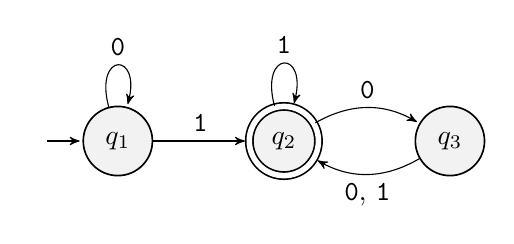
\begin{tikzpicture}
\node[state, initial] (q1) {$q_1$};
\node[state, accepting, right of=q1] (q2) {$q_2$};
\node[state, right of=q2] (q3) {$q_3$};
\draw (q1) edge[loop above] node {\tt 0} (q1);
\draw (q1) edge node {\tt 1} (q2);
\draw (q2) edge[loop above] node {\tt 1} (q2);
\draw (q2) edge[bend left] node {\tt 0} (q3);
\draw (q3) edge[bend left] node {{\tt 0}, {\tt 1}} (q2);
\end{tikzpicture}

\paragraph{NFA syntax}
\begin{grammar}
<NFA> ::= <nfa-line>*

<nfa-line> ::= <input-symbols>
  \alt <epsilon>
  \alt <states>
  \alt <initial> 
  \alt <final> 
  \alt <nfa-transition>

<nfa-transition> ::= <state> <state> <nfa-update>*

<nfa-update> ::= <symbol> <symbol> ',' <symbol>
\end{grammar}

The elements \synt{input-symbols} and \synt{states} are optional. If they are omitted, they are derived from the transitions. If \synt{epsilon} is omitted, the symbol '-' is treated as $\varepsilon$. An \synt{nfa-update} must be a single token, i.e. it may not contain spaces.

For example, the NFA below is specified using

\begin{verbatim}
initial 1
final 1
1 2 b
1 3 _
2 2 a
2 3 a b
3 1 a
\end{verbatim}

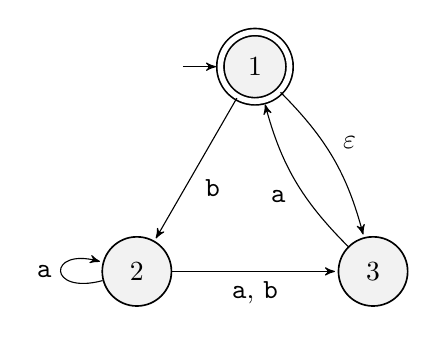
\begin{tikzpicture}
\node[state, initial, accepting] (1) at (1.5,2.6) {$1$};
\node[state] (2) at (0,0) {$2$};
\node[state] (3) at (3,0) {$3$};
\draw (1) edge node{\tt b} (2)
          edge[bend left=15] node {$\varepsilon$} (3)
      (2) edge[loop left] node{\tt a} (2)
          edge[below] node{{\tt a}, {\tt b}} (3)
      (3) edge[bend left=15] node{\tt a} (1);
\end{tikzpicture}

\paragraph{PDA syntax}
\begin{grammar}
<PDA> ::= <pda-line>*

<pda-line> ::= <input-symbols>
  \alt <stack-symbols>
  \alt <epsilon>
  \alt <states>
  \alt <initial> 
  \alt <final> 
  \alt <pda-transition>

<pda-transition> ::= <state> <state> <pda-update>*

<pda-update> ::= <symbol> ',' <symbol> <symbol>
\end{grammar}

The elements \synt{input-symbols}, \synt{stack-symbols} and \synt{states} are optional. If they are omitted, they are derived from the transitions. If \synt{epsilon} is omitted, the symbol '-' is treated as the empty string. A \synt{pda-update} must be a single token, i.e. it may not contain spaces.

For example, the PDA below is specified using

\begin{verbatim}
initial q1
final q1 q4
states q1 q2 q3 q4 q5
input_symbols 0 1
epsilon _
q1 q2 _,_$
q2 q2 0,_0
q2 q3 1,0_
q3 q3 1,0_
q3 q4 _,$_
\end{verbatim}

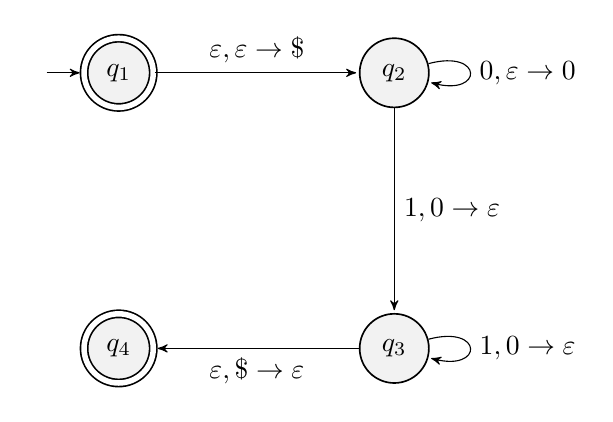
\begin{tikzpicture}[align=center,node distance=3.5cm]
\node[state, initial, accepting] (q1) {$q_1$};
\node[state, right of=q1] (q2) {$q_2$};
\node[state, below of=q2] (q3) {$q_3$};
\node[state, accepting, below of=q1] (q4) {$q_4$};
\draw (q1) edge node {\tt $\varepsilon, \varepsilon \rightarrow \$$} (q2);
\draw (q2) edge[loop right] node {\tt $0, \varepsilon \rightarrow 0$} (q2);
\draw (q2) edge node {\tt $1, 0 \rightarrow \varepsilon$} (q3);
\draw (q3) edge[loop right] node {\tt $1, 0 \rightarrow  \varepsilon$} (q3);
\draw (q3) edge node {\tt $\varepsilon, \$ \rightarrow \varepsilon$} (q4);
\end{tikzpicture}

\paragraph{Turing machine syntax}
\begin{grammar}
<TM> ::= <tm-line>*

<tm-line> ::= <input-symbols>
  \alt <tape-symbols>
  \alt <blank>
  \alt <states>
  \alt <initial> 
  \alt <accept> 
  \alt <reject> 
  \alt <tm-transition>

<tm-transition> ::= <state> <state> <tm-update>*

<tm-update> ::= <symbol> <symbol>  ',' <direction>
\end{grammar}

The elements \synt{input-symbols}, \synt{tape-symbols} and \synt{states} are optional. If they are omitted, they are derived from the transitions. If \synt{blank} is omitted, the symbol '-' is treated as the blank symbol. A \synt{tm-update} must be a single token, i.e. it may not contain spaces.

For example, the Turing machine below is specified using

\begin{verbatim}
initial q1
accept q_accept
reject q_reject
input_symbols 0
tape_symbols 0 x _
blank _
q1 q2 0_,R
q1 q_reject __,R xx,R
q2 q2 xx,R
q2 q3 0x,R
q2 q_accept __,R
q3 q3 xx,R
q3 q4 00,R
q3 q5 __,L
q4 q3 0x,R
q4 q4 xx,R
q4 q_reject __,R
q5 q2 __,R
q5 q5 00,L xx,L
\end{verbatim}

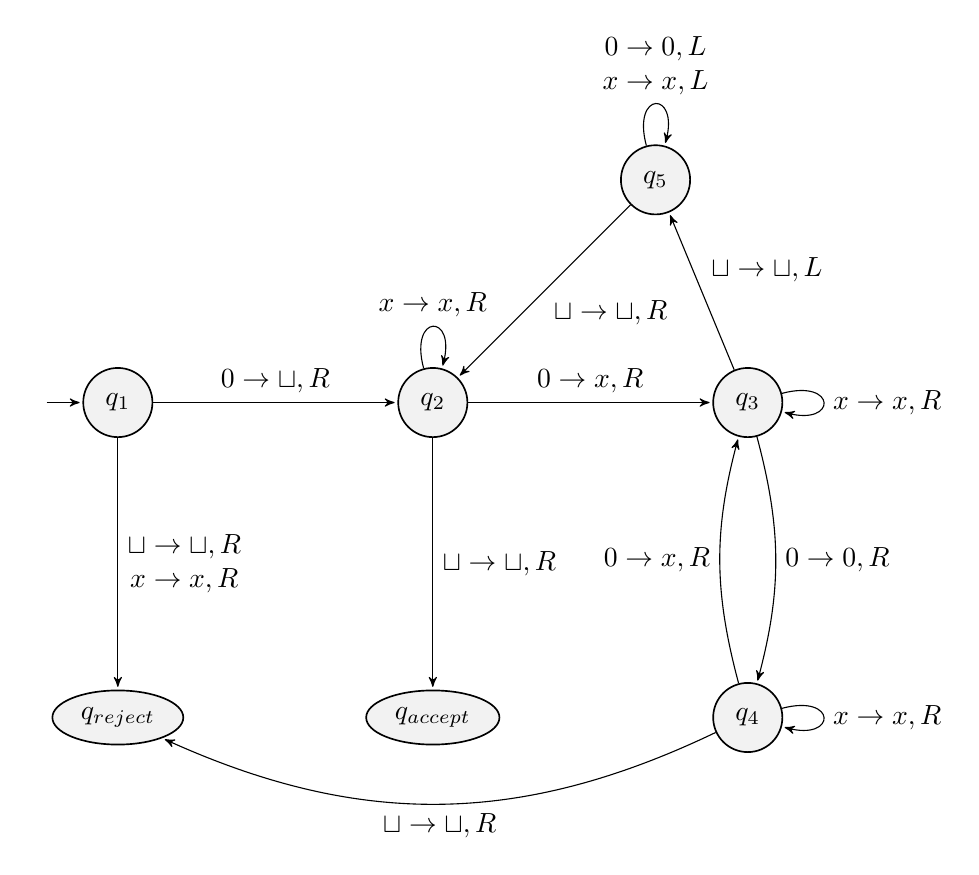
\begin{tikzpicture}[align=center,node distance=4cm]
\node[state, initial] (q1) {$q_1$};
\node[state, right of=q1] (q2) {$q_2$};
\node[state, right of=q2] (q3) {$q_3$};
\node[elliptic state, below of=q1] (qreject) {$q_{reject}$};
\node[elliptic state, below of=q2] (qaccept) {$q_{accept}$};
\node[state, below of=q3] (q4) {$q_4$};
\node[state, above right of=q2] (q5) {$q_5$};
\draw (q1) edge node {$0 \rightarrow \blank,R$} (q2);
\draw (q1) edge node {$\blank \rightarrow \blank,R$ \\ $x \rightarrow x,R$} (qreject);

\draw (q2) edge[loop above] node {$x \rightarrow x, R$} (q2);
\draw (q2) edge node {$0 \rightarrow x, R$} (q3);
\draw (q2) edge node {$\blank \rightarrow \blank,R$} (qaccept);

\draw (q3) edge[loop right] node {$x \rightarrow x, R$} (q3);
\draw (q3) edge[bend left=15] node {$0 \rightarrow 0, R$} (q4);
\draw (q3) edge[swap] node {$\blank \rightarrow \blank,L$} (q5);

\draw (q4) edge[loop right] node {$x \rightarrow x, R$} (q4);
\draw (q4) edge[bend left=15] node {$0 \rightarrow x, R$} (q3);
\draw (q4) edge[bend left=25] node {$\blank \rightarrow \blank,R$} (qreject);

\draw (q5) edge[loop above] node {$0 \rightarrow 0, L$ \\ $x \rightarrow x, L$} (q5);
\draw (q5) edge node {$\blank \rightarrow \blank,R$} (q2);
\end{tikzpicture}

\paragraph{CFG syntax}
\begin{grammar}
<CFG> ::= <rule> (';' <rule>)* ;

<rule> ::= <variable> `->' <alternative> (`|' <alternative>)* ;

<alternative> ::= <cfg-symbol> (`.' <cfg-symbol>)* ;

<variable> ::= <cfg-identifier> ;

<cfg-symbol> ::= <cfg-identifier> | `_' ;
\end{grammar}

A \synt{cfg-identifier} is a token defined by the regular expression
\mbox{\texttt{[a-zA-Z_][a-zA-Z_0-9']*}}. The left hand side of the first rule is the start variable.

\paragraph{Regular expression syntax}
\begin{grammar}
<regexp> ::= `0'
  \alt `1'
  \alt <identifier>
  \alt <regexp> `*'
  \alt <regexp> `.' <regexp>
  \alt <regexp> `+' <regexp>
  \alt `(' <regexp> `)'
\end{grammar}
The productions are ordered by priority of the operators. There is a second version of the grammar in which the concatenation symbol `.' is omitted.

\clearpage
\bibliographystyle{plain}
\bibliography{main}

\end{document}
